\chapter{Tanah yang Hidup}\label{ch:b2:living-soil}

Buku terakhir Charles Darwin, yang terbit setahun sebelum ia wafat,
membahas \omterm{prop:b2:living-soil:community}{cacing tanah}. Ia telah menaruh sebuah penanda kapur pada
sebuah ladang di dekat rumahnya pada tahun 1842 lalu menggalinya pada
tahun 1871: penandanya terbaring delapan belas sentimeter di bawah,
terkubur kotoran yang telah dibawa cacingnya ke permukaan pada sebuah
laju yang ia ukur, ia timbang, dan ia kalikan --- sepuluh ton \omterm{def:b2:living-soil:soil}{tanah}
tiap acre tiap tahun melewati tubuhnya, sehingga ``seluruh lapisan
gembur permukaan pada hamparan seluas apa pun telah lewat, dan akan
lewat lagi, tiap beberapa tahun lewat tubuh cacing.'' Dengan kata lain,
\omterm{def:b2:living-soil:soil}{tanahnya} bukanlah sebuah alas yang makhluk hidup berdiri di atasnya
melainkan sesuatu yang dibuat makhluk hidup. Bab ini membahas
pembuatan itu: bagaimana batuan menjadi \omterm{def:b2:living-soil:soil}{tanah} dan seberapa lambat,
siapa yang hidup di dalamnya dan berapa banyak, bagaimana bahan yang
mati diurai dan apa yang tersisa, bagaimana akar tumbuhan menawar
dengan jamur dan bakteri untuk apa yang tidak dapat ia peroleh
sendirian, dan seberapa cepat sebuah \omterm{def:b2:living-soil:soil}{tanah} yang perlu sepuluh ribu
tahun untuk dibangun dapat hilang.

\section{Apa itu tanah}

\begin{definition}[Tanah dan horizonnya]\label{def:b2:living-soil:soil}
\index{tanah}\index{horizon tanah}\index{humus}\index{pelapukan}\index{pedogenesis}
\emph{Tanah} adalah lapisan bahan mineral yang lapuk, bahan organik,
air, udara, dan jasad yang menutupi daratan dan menopang tumbuhan:
kira-kira separuh volumenya adalah pori, yang terisi air atau udara
dalam perbandingan yang berubah-ubah, dan separuh padatnya adalah butir
mineral --- pasir (\qtyrange{0.05}{2}{mm}), lanau
(\qtyrange{2}{50}{\micro m}), dan lempung (di bawah
\qty{2}{\micro m}), yang perbandingannya memberikan \emph{teksturnya}
--- beserta beberapa persen bahan organik yang mengatur sebagian besar
sifatnya. Sebuah penampang tanah memperlihatkan \emph{horizon}:
horizon \emph{O} berisi seresah dan bahan organik yang sebagian melapuk
di permukaannya; horizon \emph{A} yang gelap berisi tanah mineral yang
tercampur \emph{humus}, yaitu sisa penguraian yang mantap, gelap, dan
koloid; horizon \emph{B} di bawahnya, yang ke dalamnya lempung, besi,
dan bahan terlarut tercuci lalu menimbun; horizon \emph{C} berisi
batuan induk yang lapuk; dan batuan dasarnya. Sebuah tanah dibuat
(\emph{pedogenesis}) oleh lima faktor --- bahan induk, iklim, jasad,
topografi, dan waktu --- dan ia dibuat dengan lambat: pelapukannya
menghasilkan sekitar \qty{0.1}{mm} tanah tiap tahun, sehingga satu
meter tanah adalah sepuluh ribu tahun kerja.
\end{definition}

\begin{omfigure}
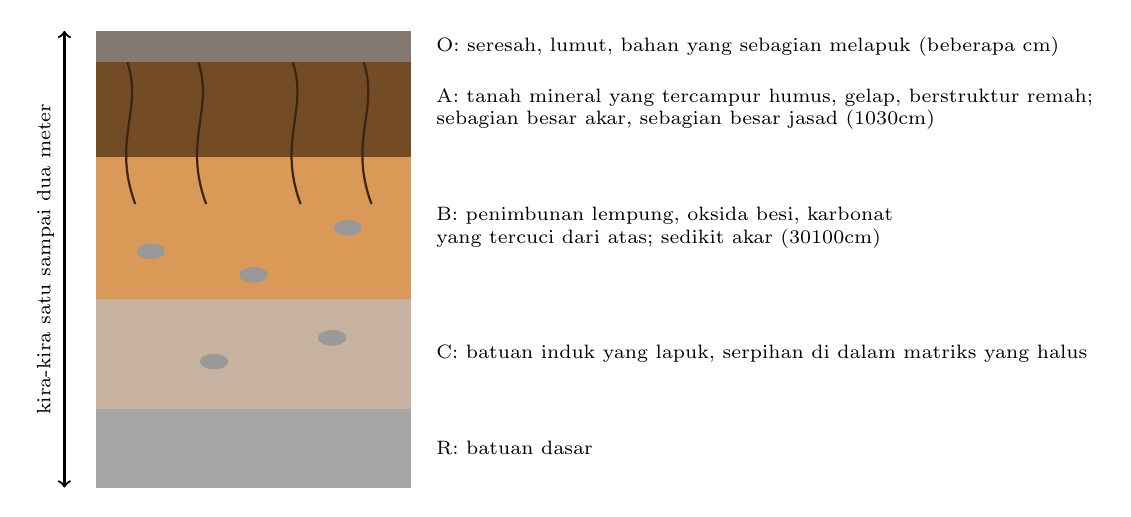
\begin{tikzpicture}[every node/.style={font=\scriptsize}]
  \fill[brown!25!black!60] (0,5.4) rectangle (4,5.8); \node[right] at (4.2,5.6) {O: seresah, lumut, bahan yang sebagian melapuk (beberapa cm)};
  \fill[brown!60!black] (0,4.2) rectangle (4,5.4); \node[right, align=left] at (4.2,4.8) {A: tanah mineral yang tercampur humus, gelap, berstruktur remah;\\ sebagian besar akar, sebagian besar jasad (\qtyrange{10}{30}{cm})};
  \fill[brown!70!orange!80] (0,2.4) rectangle (4,4.2); \node[right, align=left] at (4.2,3.3) {B: penimbunan lempung, oksida besi, karbonat\\ yang tercuci dari atas; sedikit akar (\qtyrange{30}{100}{cm})};
  \fill[gray!50!brown!60] (0,1.0) rectangle (4,2.4); \node[right, align=left] at (4.2,1.7) {C: batuan induk yang lapuk, serpihan di dalam matriks yang halus};
  \fill[gray!70] (0,0) rectangle (4,1.0); \node[right] at (4.2,0.5) {R: batuan dasar};
  \foreach \x in {0.4,1.3,2.5,3.4} \draw[brown!30!black, thick] (\x,5.4) .. controls (\x+0.2,4.8) and (\x-0.2,4.4) .. (\x+0.1,3.6);
  \foreach \x/\y in {0.7/3.0, 2.0/2.7, 3.2/3.3, 1.5/1.6, 3.0/1.9} \fill[gray!80] (\x,\y) ellipse (0.18 and 0.1);
  \draw[<->, thick] (-0.4,5.8) -- (-0.4,0) node[midway, left, rotate=90, anchor=south] {kira-kira satu sampai dua meter};
\end{tikzpicture}

{\small Sebuah penampang \omterm{def:b2:living-soil:soil}{tanah}. Bahan organiknya masuk di atasnya lalu
dihabiskan ketika ia turun; bahan mineralnya dilepaskan di bawahnya
lalu dipindahkan ke atas oleh akar dan hewan; bahan terlarutnya
berjalan turun bersama airnya lalu tertangkap di horizon B-nya.}
\end{omfigure}

\begin{proposition}[Mengapa lempung dan humus berarti]\label{prop:b2:living-soil:cec}
\index{kapasitas tukar kation}\index{lempung}\index{struktur tanah}\index{kapasitas lapang}
Partikel lempung dan \omterm{def:b2:living-soil:soil}{humus} membawa muatan negatif pada permukaannya
lalu menahan, lewat tarikan elektrostatik, sebuah cadangan kation yang
dapat ditukar --- $\mathrm{Ca^{2+}}$, $\mathrm{Mg^{2+}}$,
$\mathrm{K^{+}}$, $\mathrm{NH_4^{+}}$ --- yang diambil akar tumbuhan
dengan menukarkan $\mathrm{H^{+}}$ untuknya. \emph{\omterm{prop:b2:living-soil:cec}{Kapasitas tukar
kation}} ini adalah bank hara \omterm{def:b2:living-soil:soil}{tanahnya}; sebuah pasir nyaris tidak
memilikinya (beberapa sentimol muatan tiap kilogram), sebuah lempung
berdebu yang kaya \omterm{def:b2:living-soil:soil}{humus} lima puluh kali lebih banyak, dan kesuburan
keduanya berbeda sesuai dengan itu. Permukaan yang sama menahan air:
sebuah \omterm{def:b2:living-soil:soil}{tanah} berpasir mengering dalam sehari sampai sebuah
\emph{\omterm{prop:b2:living-soil:cec}{kapasitas lapang}} sebesar sepersepuluh volumenya, sebuah lempung
berdebu menahan sepertiga, dan selisihnya adalah apa yang dimiliki
sebuah tanaman di antara hujannya. Dan \omterm{def:b2:living-soil:soil}{humus}, bersama hifa jamur,
eksudat akar, dan lendir cacing, merekatkan butir mineralnya menjadi
\emph{agregat}, yaitu struktur remah yang porinya membiarkan udara,
air, dan akar lewat --- yaitu sifat yang membedakan sebuah \omterm{def:b2:living-soil:soil}{tanah} dari
sebuah endapan dan yang pertama kali dimusnahkan pembajakan dan
pemadatan.
\end{proposition}

\section{Siapa yang hidup di sana}

\begin{proposition}[Masyarakat tanahnya]\label{prop:b2:living-soil:community}
\index{jaring makanan tanah}\index{detritivor}\index{cacing tanah}\index{biomassa tanah}
Segram \omterm{def:b2:living-soil:soil}{tanah} atas yang subur menahan kira-kira $10^{9}$ sel bakteri
dari sekitar sepuluh ribu spesies, seratus meter hifa jamur, $10^{4}$
\omterm{def:b2:unicellular-diversity:protist}{protista}, beberapa lusin nematoda, dan segenggam tungau serta ekor
pegas; satu meter persegi menahan beberapa ratus \omterm{prop:b2:living-soil:community}{cacing tanah} dan, di
bawah hewan yang kasatmata, sebuah massa hidup sebesar beberapa ton
tiap hektar --- yang sebanding dengan sapi yang dapat ditanggung hektar
yang sama. Masyarakatnya adalah sebuah \emph{jaring makanan detritus}:
bakteri dan jamur (yaitu \emph{penguraianya}) memakan bahan yang mati
lalu dimakan \omterm{def:b2:unicellular-diversity:protist}{protista} dan nematoda (yaitu perumput mikrobanya), yang
dimakan tungau dan nematoda pemangsa, yang memberi makan kelabang dan
kumbang; \emph{detritivornya} --- \omterm{prop:b2:living-soil:community}{cacing tanah}, kaki seribu, kutu
\omterm{def:b2:plant-meristems:wood}{kayu}, rayap, ekor pegas --- memakan seresahnya sendiri beserta mikroba
padanya, lalu memecahnya seribu kali lipat dan melipatkan permukaan
yang diserang mikrobanya. Perumputnya berarti melampaui jumlahnya:
dengan memakan bakteri ia melepaskan nitrogen yang terkunci di dalam
sel bakterinya sebagai amonium, dan sebuah \omterm{def:b2:living-soil:soil}{tanah} berisi \omterm{def:b2:unicellular-diversity:protist}{protista} dan
nematoda memineralkan nitrogen lebih cepat daripada \omterm{def:b2:living-soil:soil}{tanah} yang hanya
berisi bakteri. \omterm{prop:b2:living-soil:community}{Cacing tanah} adalah \emph{insinyur ekosistemnya}:
liangnya adalah makropori \omterm{def:b2:living-soil:soil}{tanahnya}, kotorannya adalah agregat yang
terkaya, dan cacing sebuah padang rumput memindahkan beberapa ton \omterm{def:b2:living-soil:soil}{tanah}
tiap hektar lewat ususnya tiap tahun, sebagaimana diukur Darwin.
\end{proposition}

\begin{omfigure}
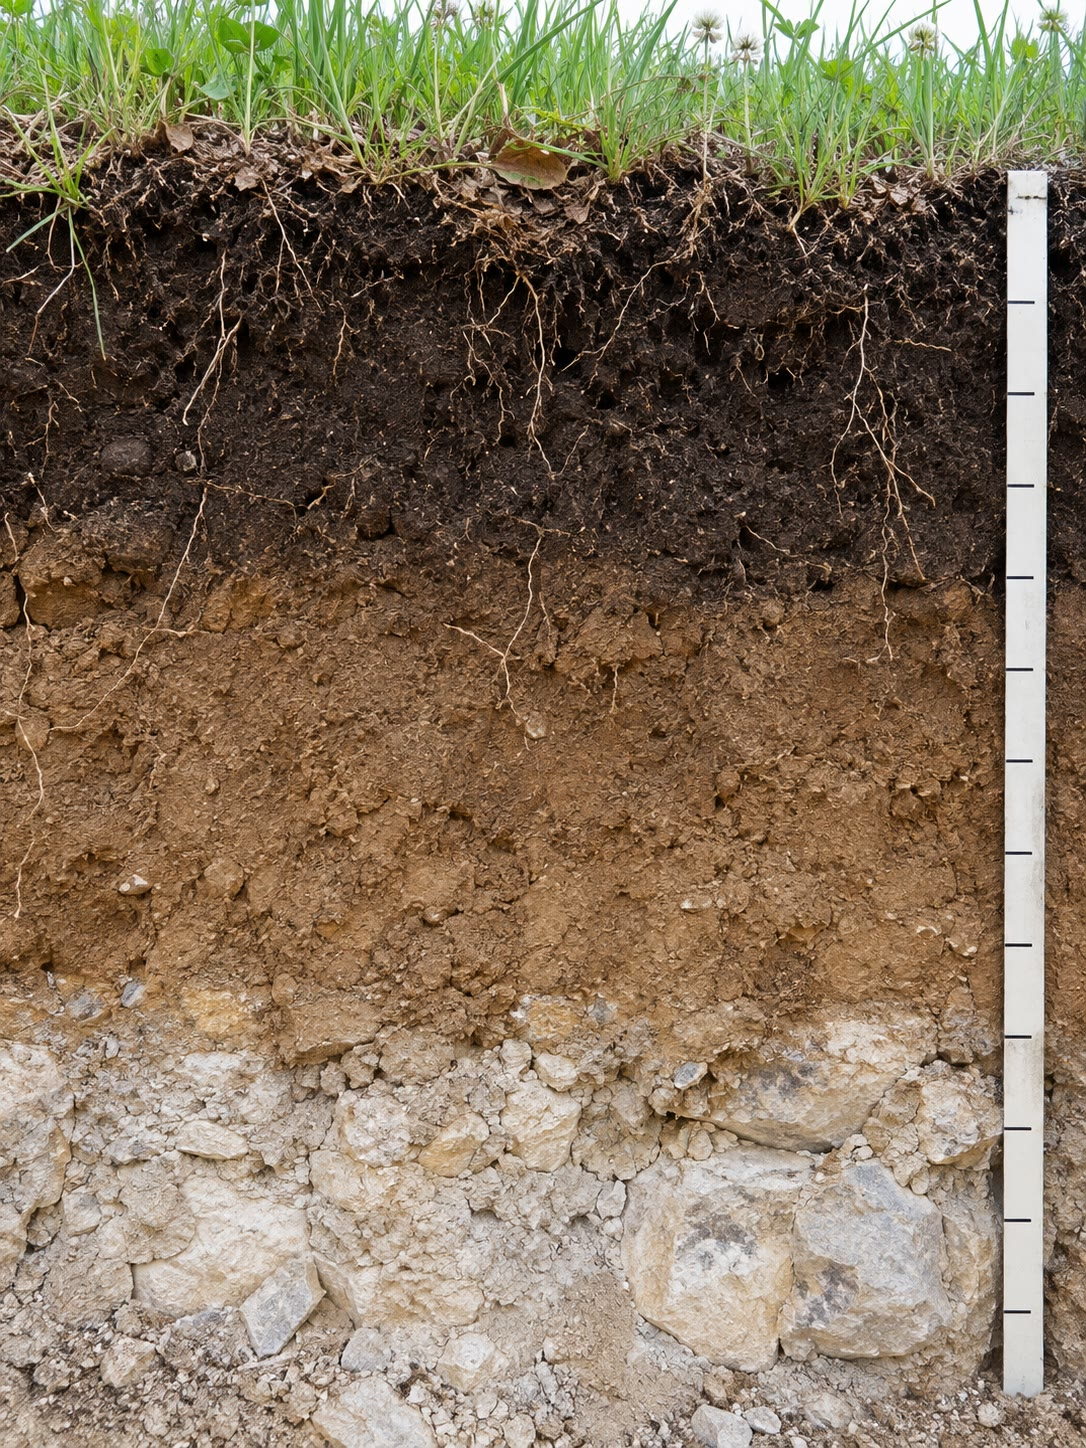
\includegraphics[width=0.21\linewidth]{images/book4/ai/b4-26-soil-profile.jpg}\hspace{0.025\linewidth}
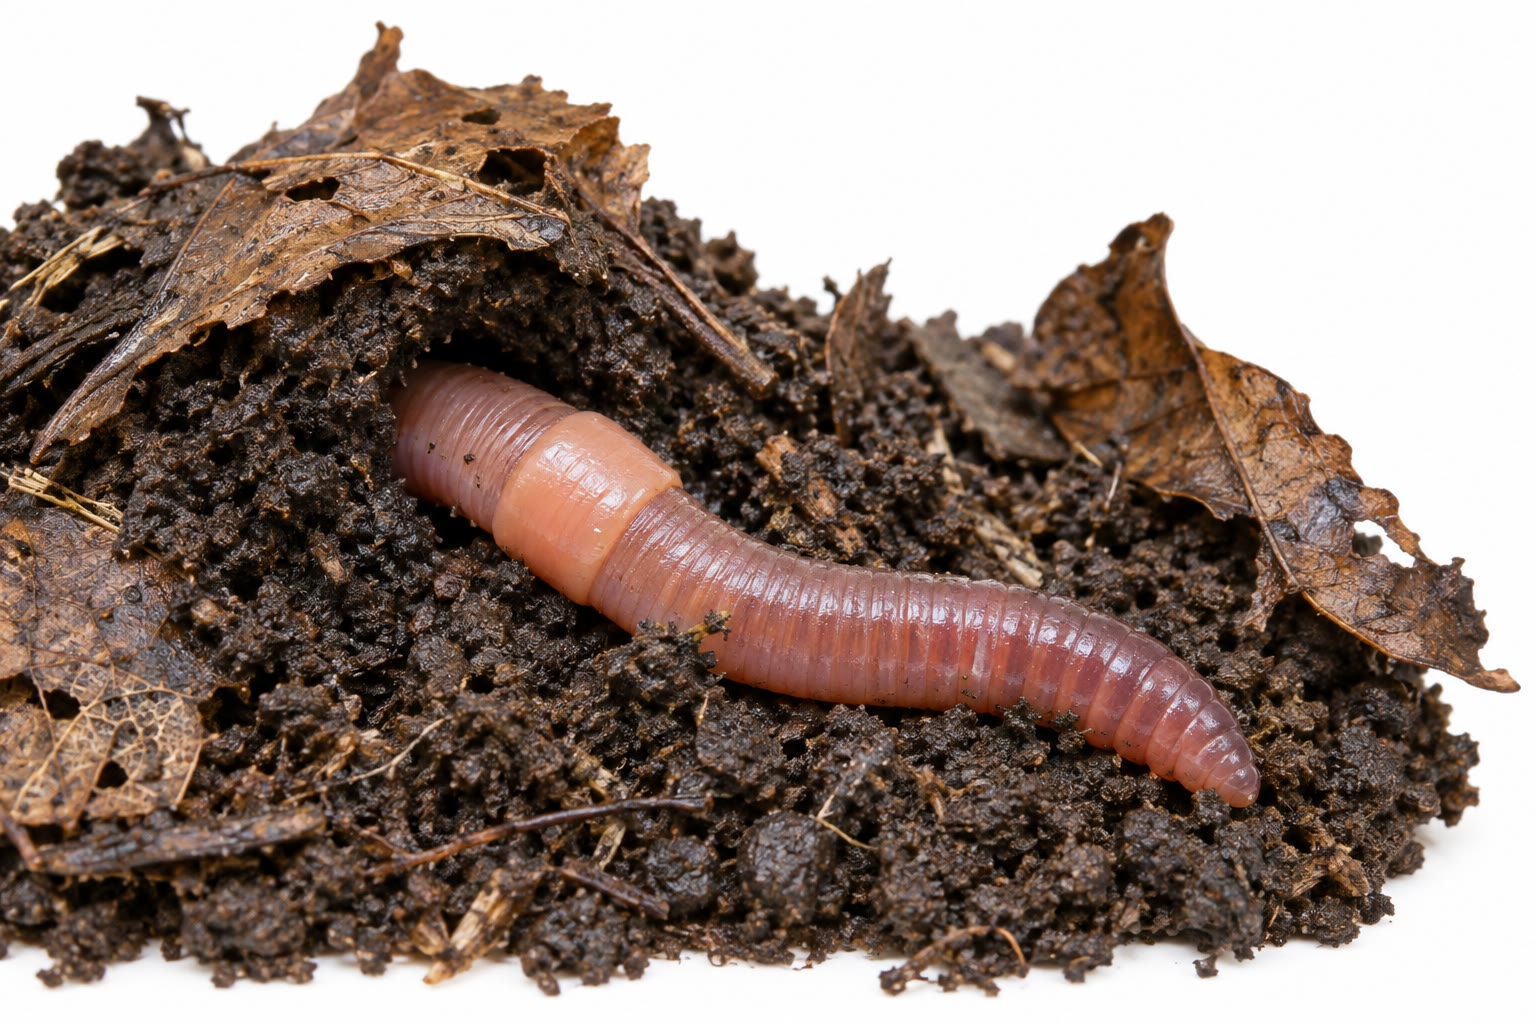
\includegraphics[width=0.42\linewidth]{images/book4/ai/b4-26-earthworm.jpg}\hspace{0.025\linewidth}
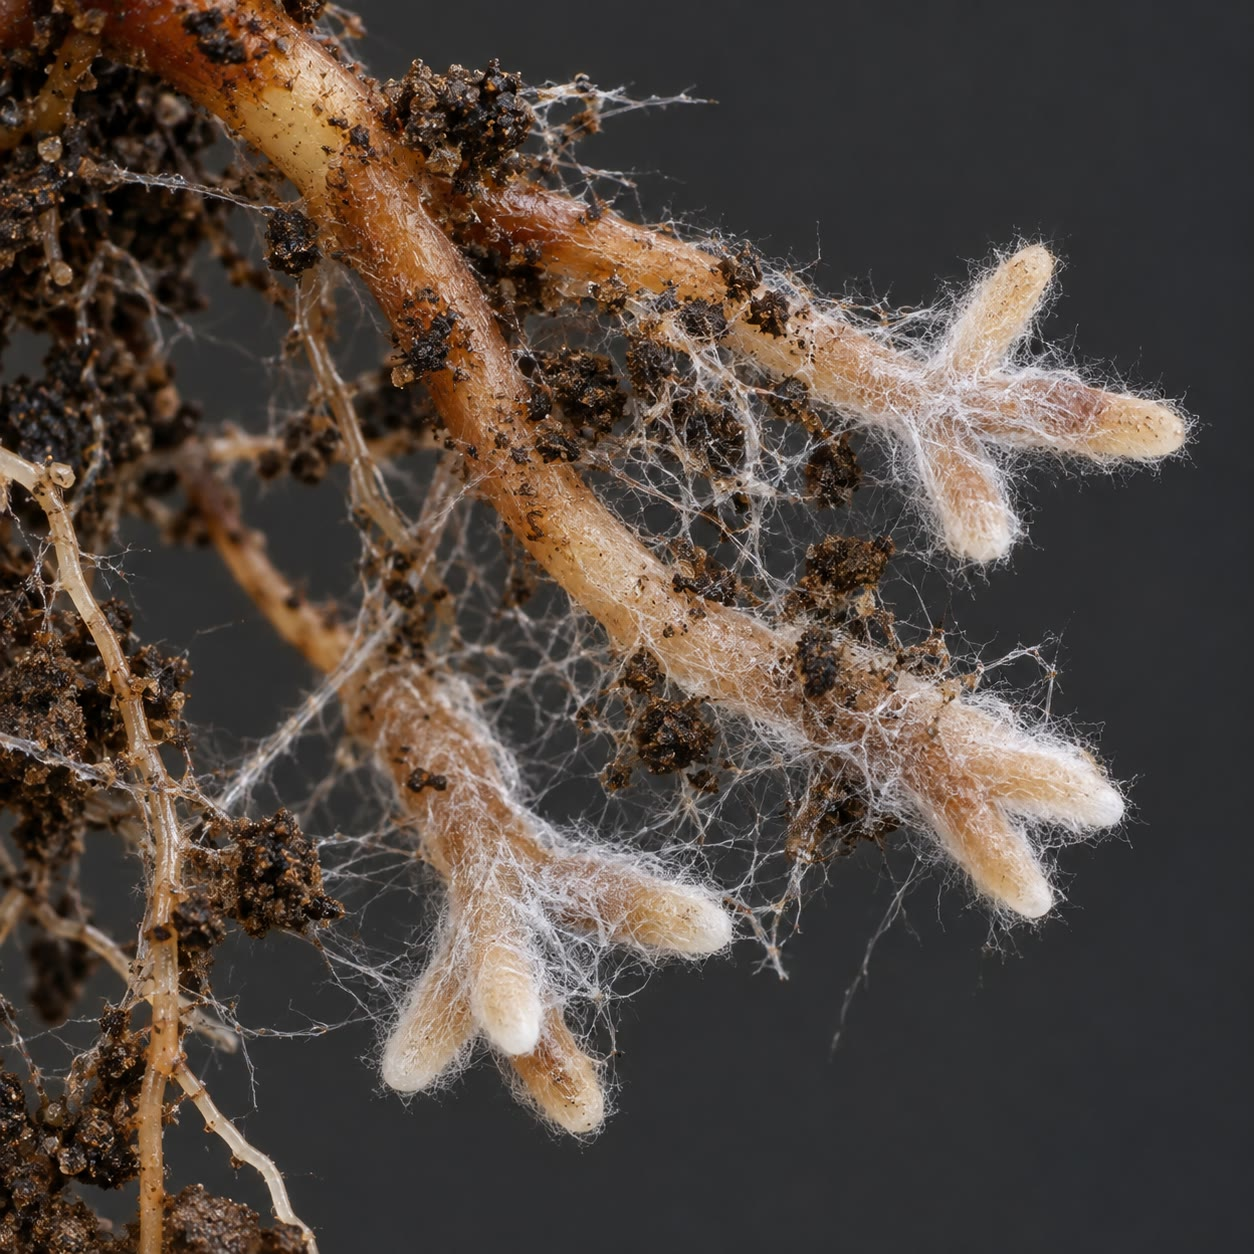
\includegraphics[width=0.28\linewidth]{images/book4/ai/b4-26-mycorrhiza.jpg}

{\small \omterm{def:b2:living-soil:soil}{Tanahnya} dan dua pembuatnya. Kiri: sebuah penampang pada
sebuah tebing potongan, \omterm{def:b2:living-soil:soil}{tanah} atas yang gelap berjenjang turun menjadi
batuan lapuk yang pucat. Tengah: seekor \omterm{prop:b2:living-soil:community}{cacing tanah} di dalam liangnya.
Kanan: sebuah akar beserta seludang ektomikorizanya dan hifa yang
memperpanjangnya ke dalam \omterm{def:b2:living-soil:soil}{tanahnya}.}
\end{omfigure}

\section{Penguraian}

\begin{theorem}[Peluruhan seresah dan nisbah karbon terhadap nitrogen]\label{thm:b2:living-soil:decay}
\index{penguraian}\index{peluruhan seresah}\index{nisbah C:N}\index{mineralisasi}\index{imobilisasi}
Seresah terurai pada laju yang sebanding dengan apa yang tersisa,
$\mathrm{d}L/\mathrm{d}t = -kL$, sehingga $L = L_0 e^{-kt}$ dengan
sebuah \emph{tetapan peluruhan} $k$ sebesar kira-kira 1 tiap tahun bagi
rumput dan daun luruh di sebuah hutan iklim sedang, $0.3$ bagi jarum
konifer, beberapa tiap tahun di tropika yang basah, dan $0.05$ di
tundranya; sebuah masukan tetap $I$ tiap tahun membangun sebuah lapisan
seresah sebesar $I/k$. Peluruhannya dikendalikan suhu, kelembapan, dan
\emph{mutu} seresahnya: kandungan nitrogennya, kandungan ligninnya, dan
nisbah karbon terhadap nitrogennya. Mikroba memiliki $\mathrm{C:N} \approx 8$ dan menahan kira-kira \qty{40}{\%} karbon yang ia makan,
sehingga ia memerlukan satu nitrogen bagi tiap $8/0.4 = 20$ karbon
makanannya: seresah dengan $\mathrm{C:N}$ di bawah kira-kira 25
melepaskan amonium ketika ia terurai (\emph{mineralisasi}), sedangkan
seresah di atasnya --- jerami pada 80, \omterm{def:b2:plant-meristems:wood}{kayu} pada 400 --- membuat
mikrobanya menyerap nitrogen dari \omterm{def:b2:living-soil:soil}{tanahnya} (\emph{imobilisasi}),
sehingga tumbuhannya kelaparan sampai karbonnya telah direspirasikan
habis dan nisbahnya telah turun. Itulah sebabnya jerami segar yang
dibajak masuk menekan sebuah tanaman, sebabnya sisa kacang-kacangan
memberinya makan, dan sebabnya sebuah timbunan kompos memerlukan
keduanya.
\end{theorem}
\begin{proof}
Bagi nisbahnya: mikroba yang memakan seresah dengan $c$ karbon tiap
nitrogennya mengasimilasi $0.4c$ karbon lalu, untuk membangun biomassa
pada $\mathrm{C:N} = 8$, memerlukan $0.4c/8 = c/20$ nitrogen;
seresahnya memasok 1. Jika $c < 20$ ada nitrogen yang berlebih, yang
dilepaskan sebagai amonium; jika $c > 20$ ada sebuah kekurangan yang
diambil dari \omterm{def:b2:living-soil:soil}{tanahnya}. Ambang 25 dalam praktiknya mencerminkan sebuah
daya guna penahanan yang sedikit di bawah 0.4. Bagi lapisan seresahnya:
$\mathrm{d}L/\mathrm{d}t = I - kL$ memiliki \omterm{def:b2:biogeochemical-cycles:reservoir}{keadaan tunak} $I/k$, yang
didekati dengan tetapan waktu $1/k$; \omterm{def:b2:biogeochemical-cycles:reservoir}{waktu tinggal} seresahnya adalah
$1/k$, satu tahun di sebuah hutan beech dan dua puluh di tundranya.
\end{proof}
\begin{proof}[Bukti eksperimental]
Percobaan kantong seresah --- massa daun yang diketahui di dalam
kantong jaring, yang dikubur lalu ditimbang pada selang tertentu ---
memberikan hukum eksponensialnya beserta tetapannya di tiap bioma
(Olson, 1963), dan memperlihatkan dengan ukuran jaring yang berbeda
bahwa menyingkirkan hewan \omterm{def:b2:living-soil:soil}{tanahnya} menyetengahkan lajunya: mikrobanya
mengerjakan kimianya tetapi hewannya menetapkan langkahnya. Di seluruh
sebuah benua, daun yang sama terurai dalam setahun di Georgia dan dalam
delapan tahun di Alaska, sebanding dengan evapotranspirasi
sesungguhnya, yaitu hasil kali kehangatan dan airnya.
\end{proof}

\begin{omfigure}
\begin{tikzpicture}
\begin{axis}[
  width=0.72\linewidth, height=5.6cm,
  axis x line=bottom, axis y line=left,
  xmin=0, xmax=6, ymin=0, ymax=105,
  xlabel={tahun}, ylabel={massa seresah yang tersisa (\%)},
  xlabel style={font=\small, at={(axis description cs:0.5,-0.13)}, anchor=north},
  ylabel style={font=\small},
  tick label style={font=\small},
  legend style={font=\scriptsize, at={(0.5,-0.3)}, anchor=north, draw=none, legend columns=2},
  clip=false,
]
\addplot[very thick, omDef, domain=0:6, samples=60] {100*exp(-2*x)};
\addlegendentry{daun hutan tropika, $k = 2$}
\addplot[very thick, omThm, domain=0:6, samples=60] {100*exp(-1*x)};
\addlegendentry{daun beech, $k = 1$}
\addplot[very thick, omProp, domain=0:6, samples=60] {100*exp(-0.3*x)};
\addlegendentry{jarum cemara, $k = 0.3$}
\addplot[very thick, gray, domain=0:6, samples=60] {100*exp(-0.05*x)};
\addlegendentry{lumut tundra, $k = 0.05$}
\end{axis}
\end{tikzpicture}

{\small Peluruhan eksponensial seresahnya. Separuh sehelai daun beech
lenyap dalam delapan bulan; separuh sebuah \omterm{def:b2:plant-life-cycles:moss}{lumut} tundra dalam empat
belas tahun; sisa yang tidak dapat dirampungkan mikroba maupun hewannya
menjadi \omterm{def:b2:living-soil:soil}{humus}.}
\end{omfigure}

\begin{proposition}[Humus dan lungkang karbon tanahnya]\label{prop:b2:living-soil:humus}
\index{humus}\index{karbon organik tanah}\index{respirasi tanah}
Beberapa persen karbon seresahnya lolos dari pengoksidaan yang lengkap
lalu menjadi \emph{\omterm{def:b2:living-soil:soil}{humus}}: sebuah campuran gelap dan tak berbentuk
berisi sisa mikroba, lignin yang terubah, dan senyawa tumbuhan, yang
terikat pada lempung dan besi serta terkunci di dalam agregatnya, yang
terurai dengan \omterm{def:b2:biogeochemical-cycles:reservoir}{waktu tinggal} berpuluh tahun sampai beribu tahun. \omterm{def:b2:living-soil:soil}{Humus}
adalah tempat kesuburan \omterm{def:b2:living-soil:soil}{tanahnya} berada --- sebagian besar nitrogen
dan pertukaran kationnya, separuh penahanan airnya --- dan ia adalah
lungkang karbon organik terbesar di daratannya, \qty{1700}{GtC} di
dalam satu meter teratasnya, yaitu dua kali atmosfernya. Perimbangannya
adalah masukan dikurangi peluruhan, $\mathrm{d}H/\mathrm{d}t = I_h - k_hH$: dengan $k_h \approx 0.02$ tiap tahun sebuah \omterm{def:b2:living-soil:soil}{tanah} menahan
masukan lima puluh tahun, dan perubahan apa pun --- pembajakan, yang
memecahkan agregatnya lalu mengudarai \omterm{def:b2:living-soil:soil}{humusnya}; pengeringan sebuah
gambut, yang memasukkan oksigen; pemanasan, yang menaikkan $k_h$ ---
muncul sebagai sebuah kehilangan yang berlanjut selama berpuluh tahun.
\omterm{def:b2:living-soil:soil}{Tanah} yang digarap di dunia telah kehilangan sepertiga sampai separuh
\omterm{def:b2:living-soil:soil}{humusnya} sejak \omterm{def:b2:living-soil:soil}{tanahnya} pertama kali dibuka, yaitu sekitar
\qty{100}{GtC}, dan sebuah pemanasan sebesar \qty{3}{\celsius} akan
menaikkan peluruhan sisanya sebesar sepertiga: \omterm{def:b2:living-soil:soil}{tanah} adalah
ketakpastian terbesar dalam anggaran karbon pada
\cref{ch:b2:global-change}.
\end{proposition}

\section{Kemitraan di bawah tanah}

\begin{proposition}[Mikoriza dan rizobium]\label{prop:b2:living-soil:symbiosis}
\index{mikoriza}\index{rizobium}\index{bintil akar}\index{nitrogenase}\index{leghemoglobin}
Sembilan dari sepuluh spesies tumbuhan memiliki akar yang dijajah jamur
di dalam sebuah \emph{mikoriza}: tumbuhannya memberikan gula
(sepersepuluh sampai seperlima fotosintatnya) dan jamurnya memberikan
fosfat, nitrogen, air, dan seng, yang hifanya, yang seratus kali lebih
tipis daripada sebuah akar dan memanjang seratus kali panjangnya tiap
satuan karbon, kumpulkan dari sebuah volume \omterm{def:b2:living-soil:soil}{tanah} yang tidak dapat
dijangkau akarnya --- terutama fosfat, yang berdifusi begitu lambat
lewat \omterm{def:b2:living-soil:soil}{tanah} sehingga sebuah akar menghabiskan satu milimeter
tetangganya dalam beberapa hari. Mikoriza \emph{arbuskular}, yaitu
jenis yang lebih tua, masuk ke dalam sel akarnya lalu bercabang menjadi
arbuskul tempat pertukarannya berlangsung; \emph{ektomikoriza} pohon
hutan menyeludungi ujung akarnya lalu tumbuh di antara selnya.
Kacang-kacangan melangkah lebih jauh: rizobium, yang ditarik flavonoid
akarnya, masuk lewat sebuah \omterm{prop:b2:plant-meristems:ram}{rambut akar}, dan akarnya membangun sebuah
\emph{bintil} di sekelilingnya yang di dalamnya bakterinya, sebagai
\emph{bakteroid}, memfiksasi nitrogen dengan nitrogenase --- yaitu
sebuah enzim yang begitu peka terhadap oksigen sehingga bintilnya harus
dijaga hampir anoksik oleh \emph{leghemoglobin}, yaitu sebuah
hemoglobin yang dibuat tumbuhannya, yang memberi bintilnya warna merah
mudanya dan mengantarkan oksigen kepada bakteroidnya pada sebuah
kepekatan yang terlalu rendah untuk meracuni enzimnya. Tiap mitranya
mengawasi yang lain: sebuah tumbuhan memutus gula bagi bintil yang
tidak memfiksasi apa pun, dan sebuah jamur yang mengantarkan lebih
sedikit fosfat menerima lebih sedikit karbon.
\end{proposition}
\begin{proof}[Bukti eksperimental]
Kiers dan rekannya (2011) menumbuhkan sebuah tumbuhan dengan dua mitra
jamur pada sebuah sistem akar yang terbagi lalu menawarkan fosfat
kepada satu sisinya saja: tumbuhannya menjatahkan lebih banyak karbon
kepada jamur yang memasok lebih banyak fosfat, dan jamurnya menjatahkan
lebih banyak fosfat kepada akar yang memberikan lebih banyak karbon ---
yaitu ganjaran timbal balik yang terukur dengan isotop. Bagi
rizobiumnya, bintil yang secara percobaan ditolak nitrogennya (dengan
menggantikan udaranya dengan argon dan oksigen) menerima lebih sedikit
oksigen lalu tumbuh lebih sedikit daripada bintil pada tumbuhan yang
sama yang dapat memfiksasi: tumbuhannya menghukum penipunya. Penelusuran
nitrogen-15 memperlihatkan bahwa sebuah hamparan semanggi--rumput
memindahkan sepertiga nitrogen yang difiksasi semangginya kepada
rumputnya dalam satu musim, lewat \omterm{def:b2:living-soil:soil}{tanahnya} dan lewat jaringan jamur
yang dipakai bersama.
\end{proof}

\begin{omfigure}
\begin{tikzpicture}[every node/.style={font=\scriptsize}, >=stealth]
  % root cross-section
  \fill[omThm!15] (0,0) circle (1.5); \draw[thick] (0,0) circle (1.5);
  \fill[omThm!30] (0,0) circle (0.5); \draw[thick] (0,0) circle (0.5);
  \node at (0,0) {stele};
  \node at (0,1.05) {korteks};
  % arbuscules in cortex cells
  \foreach \a in {30,150,270} { \draw[omDef, thick] ({1.0*cos(\a)},{1.0*sin(\a)}) -- ++({0.25*cos(\a+60)},{0.25*sin(\a+60)}) -- ++({0.2*cos(\a-40)},{0.2*sin(\a-40)}); \draw[omDef, thick] ({1.0*cos(\a)},{1.0*sin(\a)}) -- ++({0.25*cos(\a-60)},{0.25*sin(\a-60)}); }
  % hyphae out
  \foreach \a in {20,80,150,210,340} { \draw[omDef, thick] ({1.5*cos(\a)},{1.5*sin(\a)}) .. controls ({2.2*cos(\a+10)},{2.2*sin(\a+10)}) .. ({2.7*cos(\a-5)},{2.7*sin(\a-5)}); }
  \draw[omDef, thick] ({1.5*cos(150)},{1.5*sin(150)}) -- ({1.0*cos(150)},{1.0*sin(150)});
  \node[omDef, anchor=west, align=left] at (2.9,1.4) {hifa: selebar \qty{3}{\micro m},\\ bermeter-meter tiap sentimeter akar};
  \node[omDef, anchor=west] at (2.9,0.1) {arbuskul di dalam sebuah sel korteks};
  \draw[omDef] (2.85,0.1) -- (1.2,0.5);
  \node[anchor=north, align=center] at (0,-1.6) {akar, \qty{0.3}{mm} melintang};
  \draw[->, thick, omThm] (-1.2,-2.4) -- (1.2,-2.4) node[right] {gula ke jamurnya, \qtyrange{10}{20}{\%} fotosintatnya};
  \draw[<-, thick, omDef] (-1.2,-2.9) -- (1.2,-2.9) node[right] {fosfat, amonium, air, seng ke tumbuhannya};
  % nodule
  \begin{scope}[xshift=9.3cm]
    \draw[thick, brown!60!black] (-0.3,2.4) -- (-0.1,-0.6);
    \draw[thick, brown!60!black] (-0.1,0.3) -- (1.6,0.1);
    \fill[pink!60!red!40] (1.5,0.2) circle (0.9); \draw[thick] (1.5,0.2) circle (0.9);
    \fill[pink!80!red!60] (1.5,0.2) circle (0.55);
    \foreach \p in {(1.3,0.3),(1.6,0.0),(1.5,0.45),(1.7,0.3),(1.35,0.05)} \fill[omDef!70!black] \p ellipse (0.08 and 0.05);
    \node[anchor=north, align=center] at (1.5,-0.8) {bintil: bakteroid di dalam sel tumbuhan,\\ merah muda oleh leghemoglobin;\\ oksigennya ditahan pada \qty{10}{nM} agar\\ nitrogenase bekerja dan selnya bernapas};
    \node[anchor=south, align=center] at (-0.2,2.45) {akar kacang-kacangan};
  \end{scope}
\end{tikzpicture}

{\small Dua tawaran. Kiri: sebuah mikoriza arbuskular, gula keluar dan
fosfat masuk lewat arbuskul di dalam sel korteksnya. Kanan: sebuah
bintil kacang-kacangan, yang padanya hemoglobin tumbuhannya sendiri
menjaga oksigennya cukup rendah bagi nitrogenasenya dan cukup tinggi
bagi respirasinya.}
\end{omfigure}

\section{Kehilangan tanah}

\begin{proposition}[Erosi, garam, dan perimbangan sebuah tanah]\label{prop:b2:living-soil:erosion}
\index{erosi tanah}\index{salinisasi}\index{penggurunan}
\omterm{def:b2:living-soil:soil}{Tanah} terbentuk pada \qtyrange{0.05}{0.5}{mm} tiap tahun dan, di bawah
tumbuhan alaminya, tererosi pada laju yang kira-kira sama. Lahan yang
dibajak telanjang pada sebuah lereng kehilangan
\qtyrange{1}{10}{mm} tiap tahun kepada air dan anginnya ---
\qtyrange{10}{100}{t/ha} --- yaitu sepuluh sampai seratus kali laju
pembentukannya: sebuah \omterm{def:b2:living-soil:soil}{tanah} yang dibangun dalam sepuluh ribu tahun
disingkirkan dalam seabad, dan bersamanya \omterm{def:b2:living-soil:soil}{humus} dan hara horizon
A-nya, yaitu satu-satunya bagian yang berarti. Tanaman penutup,
terasering, pembajakan menurut kontur, dan pertanian tanpa olah \omterm{def:b2:living-soil:soil}{tanah},
yang meninggalkan sisanya di permukaan dan agregatnya tetap utuh,
mengembalikan kehilangannya mendekati laju pembentukannya. Pengairan di
iklim yang kering membawa kegagalan yang berlawanan: airnya menguap
lalu meninggalkan garamnya, satu ton tiap hektar tiap tahun dari air
yang hanya sedikit asin, sampai potensial osmosis larutan \omterm{def:b2:living-soil:soil}{tanahnya}
(\cref{ch:b2:plant-plasticity}) lebih rendah daripada yang dapat
diatasi akarnya --- yaitu \emph{salinisasi}, yang memensiunkan ladang
Sumeria empat ribu tahun yang lalu dan kini menimpa seperlima lahan
yang diairi. Keadaan sebuah \omterm{def:b2:living-soil:soil}{tanah} adalah sebuah anggaran: \omterm{def:b2:living-soil:soil}{humus} masuk
berbanding \omterm{def:b2:living-soil:soil}{humus} keluar, pembentukan berbanding erosi, garam masuk
berbanding garam yang teralirkan; masing-masingnya memiliki sebuah
\omterm{def:b2:biogeochemical-cycles:reservoir}{waktu tinggal}, dan masing-masingnya, setelah negatif, lambat untuk
dibalikkan.
\end{proposition}

\section{Latihan}

\begin{exercise}[$\star$]\label{exo:b2:living-soil:1}
Sebutkan horizon sebuah penampang \omterm{def:b2:living-soil:soil}{tanah} dari permukaannya ke bawah
lalu katakan apa yang terjadi pada masing-masingnya.
\end{exercise}

\begin{exercise}[$\star$]\label{exo:b2:living-soil:2}
Jelaskan apa itu \omterm{prop:b2:living-soil:cec}{kapasitas tukar kation}, mengapa sebuah \omterm{def:b2:living-soil:soil}{tanah} berpasir
memilikinya sedikit, dan apa yang dikerjakan seorang petani yang
mengapuri sebuah \omterm{def:b2:living-soil:soil}{tanah} yang masam terhadapnya.
\end{exercise}

\begin{exercise}[$\star$]\label{exo:b2:living-soil:3}
Sebutkan kelompok utama \omterm{prop:b2:living-soil:community}{jaring makanan tanahnya} dari penguraianya
sampai pemangsa puncaknya, beserta satu jasad masing-masingnya, lalu
katakan apa yang dikerjakan perumput bakterinya bagi tumbuhannya.
\end{exercise}

\begin{exercise}[$\star$]\label{exo:b2:living-soil:4}
Bedakan mikoriza arbuskular dan ektomikoriza, lalu nyatakan apa yang
diberikan dan diperoleh tiap mitranya.
\end{exercise}

\begin{exercise}[$\star\star$]\label{exo:b2:living-soil:5}
Sebuah hutan beech menjatuhkan \qty{4}{t/ha} daun tiap tahun dan
\omterm{thm:b2:living-soil:decay}{peluruhan seresahnya} berlangsung dengan $k = 0.8$ tiap tahun. Hitunglah massa
seresah \omterm{def:b2:biogeochemical-cycles:reservoir}{keadaan tunaknya}, \omterm{def:b2:biogeochemical-cycles:reservoir}{waktu tinggal} seresahnya, dan waktu bagi
jatuhan setahun untuk kehilangan \qty{90}{\%} massanya.
\end{exercise}

\begin{exercise}[$\star\star$]\label{exo:b2:living-soil:6}
Jerami gandum memiliki $\mathrm{C:N} = 80$ dan sisa semanggi $15$. Bagi
masing-masingnya, hitunglah nitrogen yang dibutuhkan mikrobanya tiap
\qty{100}{kg} karbon yang dihabiskan (dengan penahanan 0.4 dan
$\mathrm{C:N} = 8$ bagi mikrobanya) dan apakah sisanya memineralkan atau
mengimobilisasi, serta seberapa banyak.
\end{exercise}

\begin{exercise}[$\star\star$]\label{exo:b2:living-soil:7}
Sehektar padang rumput menahan \qty{2}{t} \omterm{prop:b2:living-soil:community}{cacing tanah} yang
masing-masing mengolah sepuluh kali massanya berupa \omterm{def:b2:living-soil:soil}{tanah} tiap tahun.
Hitunglah \omterm{def:b2:living-soil:soil}{tanah} yang lewat cacingnya tiap tahun dan waktu bagi
\qty{20}{cm} teratasnya (dengan rapat massa curah \qty{1.3}{t/m^3})
untuk lewat sekali. Bandingkan dengan angka Darwin.
\end{exercise}

\begin{exercise}[$\star\star$]\label{exo:b2:living-soil:8}
Segram \omterm{def:b2:living-soil:soil}{tanah} menahan $10^{9}$ bakteri bermassa \qty{e-12}{g}
masing-masing, dan \qty{100}{m} hifa bergaris tengah \qty{4}{\micro m}
dan berapat massa \qty{1.1}{g/cm^3}. Hitunglah biomassa bakteri dan
jamurnya tiap gram dan tiap hektar (\qty{20}{cm} teratasnya,
\qty{1.3}{t/m^3}).
\end{exercise}

\begin{exercise}[$\star\star$]\label{exo:b2:living-soil:9}
\omterm{def:b2:living-soil:soil}{Humus} \omterm{def:b2:living-soil:soil}{tanah} meluruh dengan $k_h = 0.02$ tiap tahun dan menerima
\qty{1.5}{t/ha} karbon tiap tahun. Hitunglah karbon \omterm{def:b2:living-soil:soil}{humus} \omterm{def:b2:biogeochemical-cycles:reservoir}{keadaan
tunaknya}. Ladangnya dibajak dan $k_h$ melipat dua: hitunglah \omterm{def:b2:biogeochemical-cycles:reservoir}{keadaan
tunaknya} yang baru, karbon yang hilang, dan waktu untuk kehilangan
separuhnya.
\end{exercise}

\begin{exercise}[$\star\star\star$]\label{exo:b2:living-soil:10}
Fosfat berdifusi lewat \omterm{def:b2:living-soil:soil}{tanah} dengan $D \approx \qty{e-13}{m^2/s}$.
Hitunglah seberapa jauh ia berjalan dalam sebuah musim tumbuh selama
\num{100} hari ($x \approx \sqrt{2Dt}$) lalu bandingkan dengan jarak
antarakar (\qty{1}{cm}) dan antarhifa (\qty{0.1}{mm}). Apa yang
dikatakan hal ini tentang mengapa mikoriza berarti bagi fosfor dan
kurang berarti bagi nitrat ($D \approx \qty{e-10}{m^2/s}$)?
\end{exercise}

\begin{exercise}[$\star\star\star$]\label{exo:b2:living-soil:11}
Sebuah lereng kehilangan \qty{20}{t/ha} \omterm{def:b2:living-soil:soil}{tanah} tiap tahun karena erosi
sementara membentuk \qty{1}{t/ha}; horizon A-nya setebal \qty{25}{cm}
pada \qty{1.3}{t/m^3} dan menahan karbon \qty{3}{\%}. Hitunglah massa
horizon A-nya, umurnya pada laju ini, dan karbon yang hilang tiap
tahun. Di bawah tanpa olah \omterm{def:b2:living-soil:soil}{tanah} kehilangannya turun menjadi
\qty{2}{t/ha}: hitung ulang umurnya.
\end{exercise}

\begin{exercise}[$\star\star\star$]\label{exo:b2:living-soil:12}
``\omterm{def:b2:living-soil:soil}{Tanah} adalah jasad yang paling lambat di sebuah ladang.'' Bahaslah
dengan \omterm{def:b2:biogeochemical-cycles:reservoir}{waktu tinggal} seresah, \omterm{def:b2:living-soil:soil}{humus}, \omterm{def:b2:living-soil:soil}{tanah} mineral, dan garamnya, lalu
katakan perubahan mana yang dapat dilihat seorang petani dalam satu
karier dan mana yang tidak.
\end{exercise}

\section{Soal: Sehektar Tanah}

\begin{problem}[{Soal akhir pekan --- sehektar tanah garapan diaudit:
massa hidupnya dicacah, seresah dan humusnya diikuti lewat anggaran
eksponensialnya, nitrogen yang dilepaskan sisa kacang-kacangan dihitung
terhadap kebutuhan sebuah tanaman, dan rekening erosi serta karbon dua
cara pengelolaan dibandingkan, berakhir pada stok karbon tanahnya,
umurnya di bawah bajaknya, dan nitrogen yang dipasok sebuah
kacang-kacangan}]
\label{pb:b2:living-soil:1}
Hektarnya: horizon A setebal \qty{25}{cm}, rapat massa curah
\qty{1.3}{t/m^3}, karbon organik \qty{2.5}{\%}; peluruhan \omterm{def:b2:living-soil:soil}{humus} $k_h =
0.025$ tiap tahun di bawah bajaknya, $0.015$ di bawah tanpa olah
\omterm{def:b2:living-soil:soil}{tanahnya}; masukan karbon kepada \omterm{def:b2:living-soil:soil}{humusnya} \qty{1.2}{t/ha} tiap tahun
pada keduanya. Seresahnya: sebuah tanaman penutup semanggi
meninggalkan \qty{5}{t/ha} bahan kering berisi karbon \qty{45}{\%} dan
nitrogen \qty{3}{\%}, yang meluruh dengan $k = 2$ tiap tahun. Erosinya:
\qty{15}{t/ha} tiap tahun jika dibajak, \qty{1.5}{t/ha} tanpa olah
\omterm{def:b2:living-soil:soil}{tanah}; pembentukannya \qty{0.5}{t/ha}.

\medskip
\noindent\textbf{Bagian I --- Stoknya.}
\begin{enumerate}
  \item Hitunglah massa horizon A-nya dan karbon organiknya.
  \item Hitunglah massa nitrogen di dalam \omterm{def:b2:living-soil:soil}{humusnya} jika
        $\mathrm{C:N}$-nya 12.
  \item \omterm{def:b2:living-soil:soil}{Tanahnya} menahan $10^{9}$ bakteri tiap gram pada \qty{e-12}{g}
        masing-masing dan \qty{200}{m} hifa tiap gram bergaris tengah
        \qty{4}{\micro m}, berapat massa 1.1. Hitunglah biomassa
        mikrobanya tiap hektar.
  \item Tambahkan \qty{1.5}{t/ha} \omterm{prop:b2:living-soil:community}{cacing tanah} dan \qty{0.2}{t/ha}
        hewan lainnya, lalu berikan seluruh massa hidupnya tiap hektar.
        Berapakah ia sebagai bagian dari karbon \omterm{def:b2:living-soil:soil}{humusnya}?
  \item Mikrobanya mengganti biomassanya dua kali tiap tahun lalu
        merespirasikan \qty{60}{\%} yang ia makan. Taksirlah karbon
        yang ia habiskan tiap tahun, dan $\mathrm{CO_2}$ yang
        direspirasikannya.
  \item Bandingkan dengan produksi primer bersih tanamannya yang
        kira-kira \qty{5}{t/ha} karbon lalu berilah ulasan.
\end{enumerate}

\medskip
\noindent\textbf{Bagian II --- Sisa semangginya.}
\begin{enumerate}[resume]
  \item Hitunglah karbon dan nitrogen di dalam sisanya beserta
        $\mathrm{C:N}$-nya.
  \item Dengan $\mathrm{C:N} = 8$ bagi mikrobanya dan penahanan $0.4$,
        apakah sisanya memineralkan atau mengimobilisasi nitrogen?
        Hitunglah nitrogen bersih yang dilepaskan ketika seluruh
        sisanya terurai.
  \item Dengan $k = 2$, bagian berapa dari sisanya yang telah terurai
        setelah 3 bulan? Setelah setahun?
  \item Hitunglah nitrogen yang dilepaskan pada 3 bulan pertamanya.
  \item Sebuah tanaman gandum menyerap \qty{150}{kg} nitrogen tiap
        hektar, sebagian besarnya pada dua bulan setelah penanamannya.
        Berilah ulasan tentang waktunya.
  \item Massa jerami gandum yang sama ($\mathrm{C:N} = 80$) dibajak
        masuk sebagai gantinya. Hitunglah nitrogen yang terimobilisasi
        lalu katakan apa yang harus dikerjakan petaninya.
\end{enumerate}

\medskip
\noindent\textbf{Bagian III --- \omterm{def:b2:living-soil:soil}{Humusnya}.}
\begin{enumerate}[resume]
  \item Hitunglah karbon \omterm{def:b2:living-soil:soil}{humus} \omterm{def:b2:biogeochemical-cycles:reservoir}{keadaan tunaknya} di bawah bajaknya dan
        di bawah tanpa olah \omterm{def:b2:living-soil:soil}{tanahnya}.
  \item Ladangnya, pada \omterm{def:b2:biogeochemical-cycles:reservoir}{keadaan tunak} yang dibajak, diubah menjadi
        tanpa olah \omterm{def:b2:living-soil:soil}{tanah}. Tulislah $H(t)$ lalu hitunglah karbon yang
        diperoleh setelah 10 dan 50 tahun.
  \item Hitunglah laju perolehannya pada tahun pertamanya, dalam ton
        karbon tiap hektar, dan sebagai ton $\mathrm{CO_2}$.
  \item Jika \qty{1.5e9}{ha} lahan tanaman dunia mengerjakan hal yang
        sama, berapakah lubuk tahun pertamanya, berbanding pancaran
        fosil \qty{10}{GtC}? Dan pada tahun kelima puluhnya?
  \item Mengapa lubuknya sementara dan dapat balik?
  \item Sebuah pemanasan \qty{3}{\celsius} menaikkan $k_h$ sebesar
        sepertiga. Hitunglah \omterm{def:b2:biogeochemical-cycles:reservoir}{keadaan tunak} tanpa olah \omterm{def:b2:living-soil:soil}{tanahnya} yang
        baru dan karbon yang hilang.
\end{enumerate}

\medskip
\noindent\textbf{Bagian IV --- Erosinya.}
\begin{enumerate}[resume]
  \item Hitunglah kehilangan bersih \omterm{def:b2:living-soil:soil}{tanahnya} tiap tahun di bawah tiap
        caranya.
  \item Hitunglah umur horizon A-nya di bawah masing-masingnya.
  \item Hitunglah karbon dan nitrogen yang terbawa pergi tiap tahun
        oleh erosinya di bawah bajaknya.
  \item Bandingkan kehilangan karbon erosinya dengan kehilangan
        peluruhan \omterm{def:b2:living-soil:soil}{humusnya} pada \omterm{def:b2:biogeochemical-cycles:reservoir}{keadaan tunak} di bawah bajaknya.
  \item \omterm{def:b2:living-soil:soil}{Tanah} yang tererosi diendapkan di hilirnya. Apakah karbonnya
        hilang ke atmosfernya? Bahaslah.
  \item Berikan \omterm{def:b2:biogeochemical-cycles:reservoir}{waktu tinggal} seresah, \omterm{def:b2:living-soil:soil}{humus}, dan \omterm{def:b2:living-soil:soil}{tanah} mineralnya
        pada hektar ini.
  \item Nyatakan hasilnya: stok karbon horizon A-nya, umurnya di bawah
        bajaknya dan di bawah tanpa olah \omterm{def:b2:living-soil:soil}{tanahnya}, serta nitrogen yang
        dipasok sisa semangginya.
\end{enumerate}
\end{problem}
